\chapter{相关工作}


本章将首先详细介绍量化交易实践中低延时交易系统的基本功能与组成,由此介绍多分支因子模型的设计原理与结构特征。
其次,伴随近年来大语言模型推理需求的快速增加,诞生了大量具有良好设计的开源模型推理框架,本章将介绍当前服务端主流模型推理框架的架构设计与技术应用。
最后,作为高频交易场景下因子模型推理的基础,CPU高性能计算体系将会被概略阐述。

\section{低延时交易系统}

\begin{wrapfigure}{r}{0.5\linewidth}
    \centering
    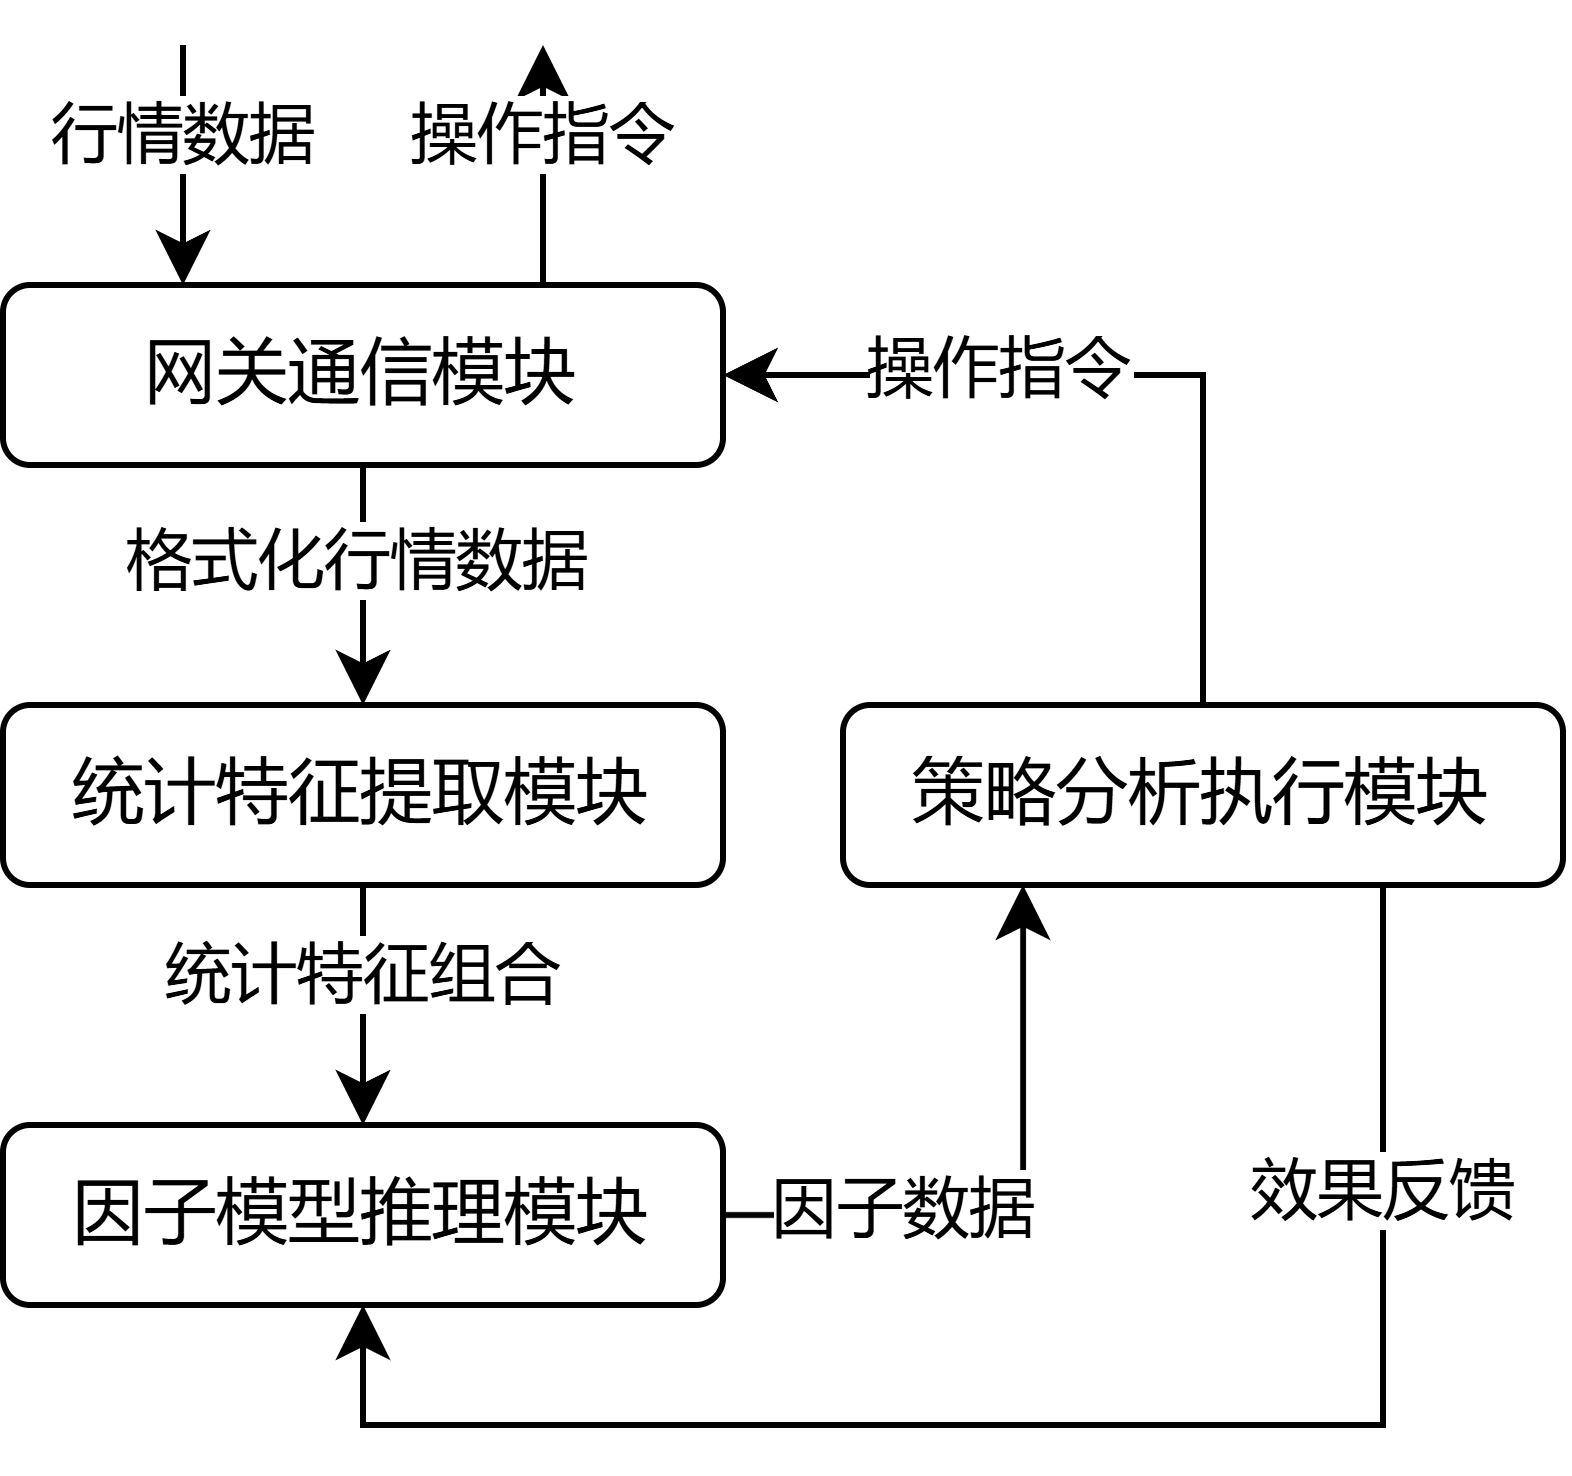
\includegraphics[width=0.5\textwidth]{image/chap02/低延时.png}
    \caption{低延时系统基本组成}
    \label{fig:image-embedding-text}
\end{wrapfigure}
低延时交易系统是量化交易的核心基础设施,其主要功能是在低延时内完成市场行情的接收、分析与交易策略的执行。
系统通常包含多个紧密协作的模块:首先是网关模块,负责快速接收和解析交易所的行情数据,确保数据的实时性与准确性;
接着是数据预处理模块,对原始行情数据进行清洗、标准化等操作,提取关键的统计特征,为后续分析奠定基础;
然后是因子模型推理模块,该模块将预处理后的特征数据输入因子模型,进行计算推理,输出作为对行情的预测;
最后是策略执行模块,依据因子模型的输出结果,迅速判断并执行具体的交易策略,如下单、撤单等操作,确保交易的高效执行,同时向因子模型反馈信息。

为了实现高频交易下极低延时的目标,低延时交易系统在设计与实现上面临着诸多严峻的技术挑战。
整个交易流程的关键路径执行时间必须被严格控制在数十微秒之内,这对系统的每个环节都提出了极高的性能要求。
为此,交易系统中的各个模块均综合了系统与硬件特性,从而尽可能降低延时。
例如,网关模块采用用户态网络库(如DPDK)与FPGA硬件加速技术,实现快速接收和解析行情数据;
数据预处理模块运用多线程并行处理与内存数据库(如Redis),或将模块编入内核态中直接完成数据清洗与标准化;
因子模型推理模块借助模型剪枝、模型压缩与优化及高效算法,提升复杂模型的推理速度;
策略执行模块则依赖高性能编程语言(如C++)、快速订单管理系统及直接市场接入(DMA)技术,确保交易策略的高效执行。
在这一过程中,因子模型的推理计算尤为关键,由于其计算复杂度高,因此在全过程延时中占有较大比例。
由此可见,优化因子模型的推理效率,降低其计算延时,成为确保交易策略能够顺利、及时执行的核心所在。
这不仅需要对因子模型本身的结构进行深入优化,还需要对推理框架的架构设计和软件算法进行全面的调整与改进,以实现整个系统的高效协同运作。



\section{因子模型}

因子模型作为量化交易的决策核心,设计的目标在于为行情建立模型,从中获取可用于策略分析的简易有效特征。
因子是能够解释资产收益变异性的特征或变量。
设计因子模型时,需从行情数据中挖掘出具有预测能力的因子,这些因子可以是基本面指标(如市盈率、市净率等),也可以是技术指标(如移动平均线、相对强弱指标等),还可以是宏观经济指标(如利率、通货膨胀率等)。
通过统计和数学方法,建立因子与资产收益之间的定量关系,以揭示因子影响资产未来收益的途径。
因子模型不仅关注收益的预测,还需考虑风险的控制。某些因子可能在带来高收益的同时伴随高风险,因此在模型设计中要找到风险与收益的最佳平衡点,实现投资者的效用最大化。


以动量因子为例,$\alpha_{i,t}$ 表示第 $i$ 个资产在时间 $t$ 的alpha因子值,$P_{t}$ 表示时间 $t$ 的资产价格,$P_{t-N}$ 表示时间 $t-N$ 的资产价格,$N$ 表示过去的时间窗口长度。
\begin{align}
    \begin{split}
        \alpha_{i,t} &= \frac{P_{t} - P_{t-N}}{P_{t-N}} \\
    \end{split}
\end{align}
此类早期因子模型主要基于经验公式,直接对行情数据的某些统计量进行数学运算,一定程度上指示交易方向,但其表征市场行情特征的能力极其有限,难以应对复杂的市场环境。
尤其是伴随经验公式中超参数的引入,其调整难度和复杂性快速增加,实际应用价值逐步下降。
随着机器学习技术的发展,因子模型逐渐使用机器学习方法提高抗噪能力和表征水平。
现代因子模型,尤其是多分支因子模型,通过多分支结构综合处理多种行情指标,能够有效捕捉市场行情的复杂特征,极大提升了模型的表征能力和抗噪性能,为交易者提供了更为精准、可靠的决策依据,从而在激烈的市场竞争中占据优势。

多分支因子模型的输入通常是多种行情特征的拼接,在输入后切片进入不同的分支进行初步处理,随后通过计算操作融合各条分支,从而使得模型可以综合不同行情特征,并最终给出因子输出指示策略执行。
从输入模式方面,多分支因子模型的输入具有高度的可拓展性,其输入既包含了多个统计特征,但是又相互独立。
这使得多分支因子模型在计算过程相互独立的分支之间可以针对各分支输入实现优化算法。
在结构特征方面,多分支因子模型其整体结构类似树状收敛,分支之间融合后形成唯一的新分支,最终汇集为模型的唯一输出。
这种结构综合分析了多个分支的特征,有效提高了模型的性能,尤其是残差连接\cite{he2015deepresiduallearningimage}大幅提高了模型设计的可用深度,多分支因子模型因此具有更强的综合能力。
\begin{figure}[h]
    \centering
    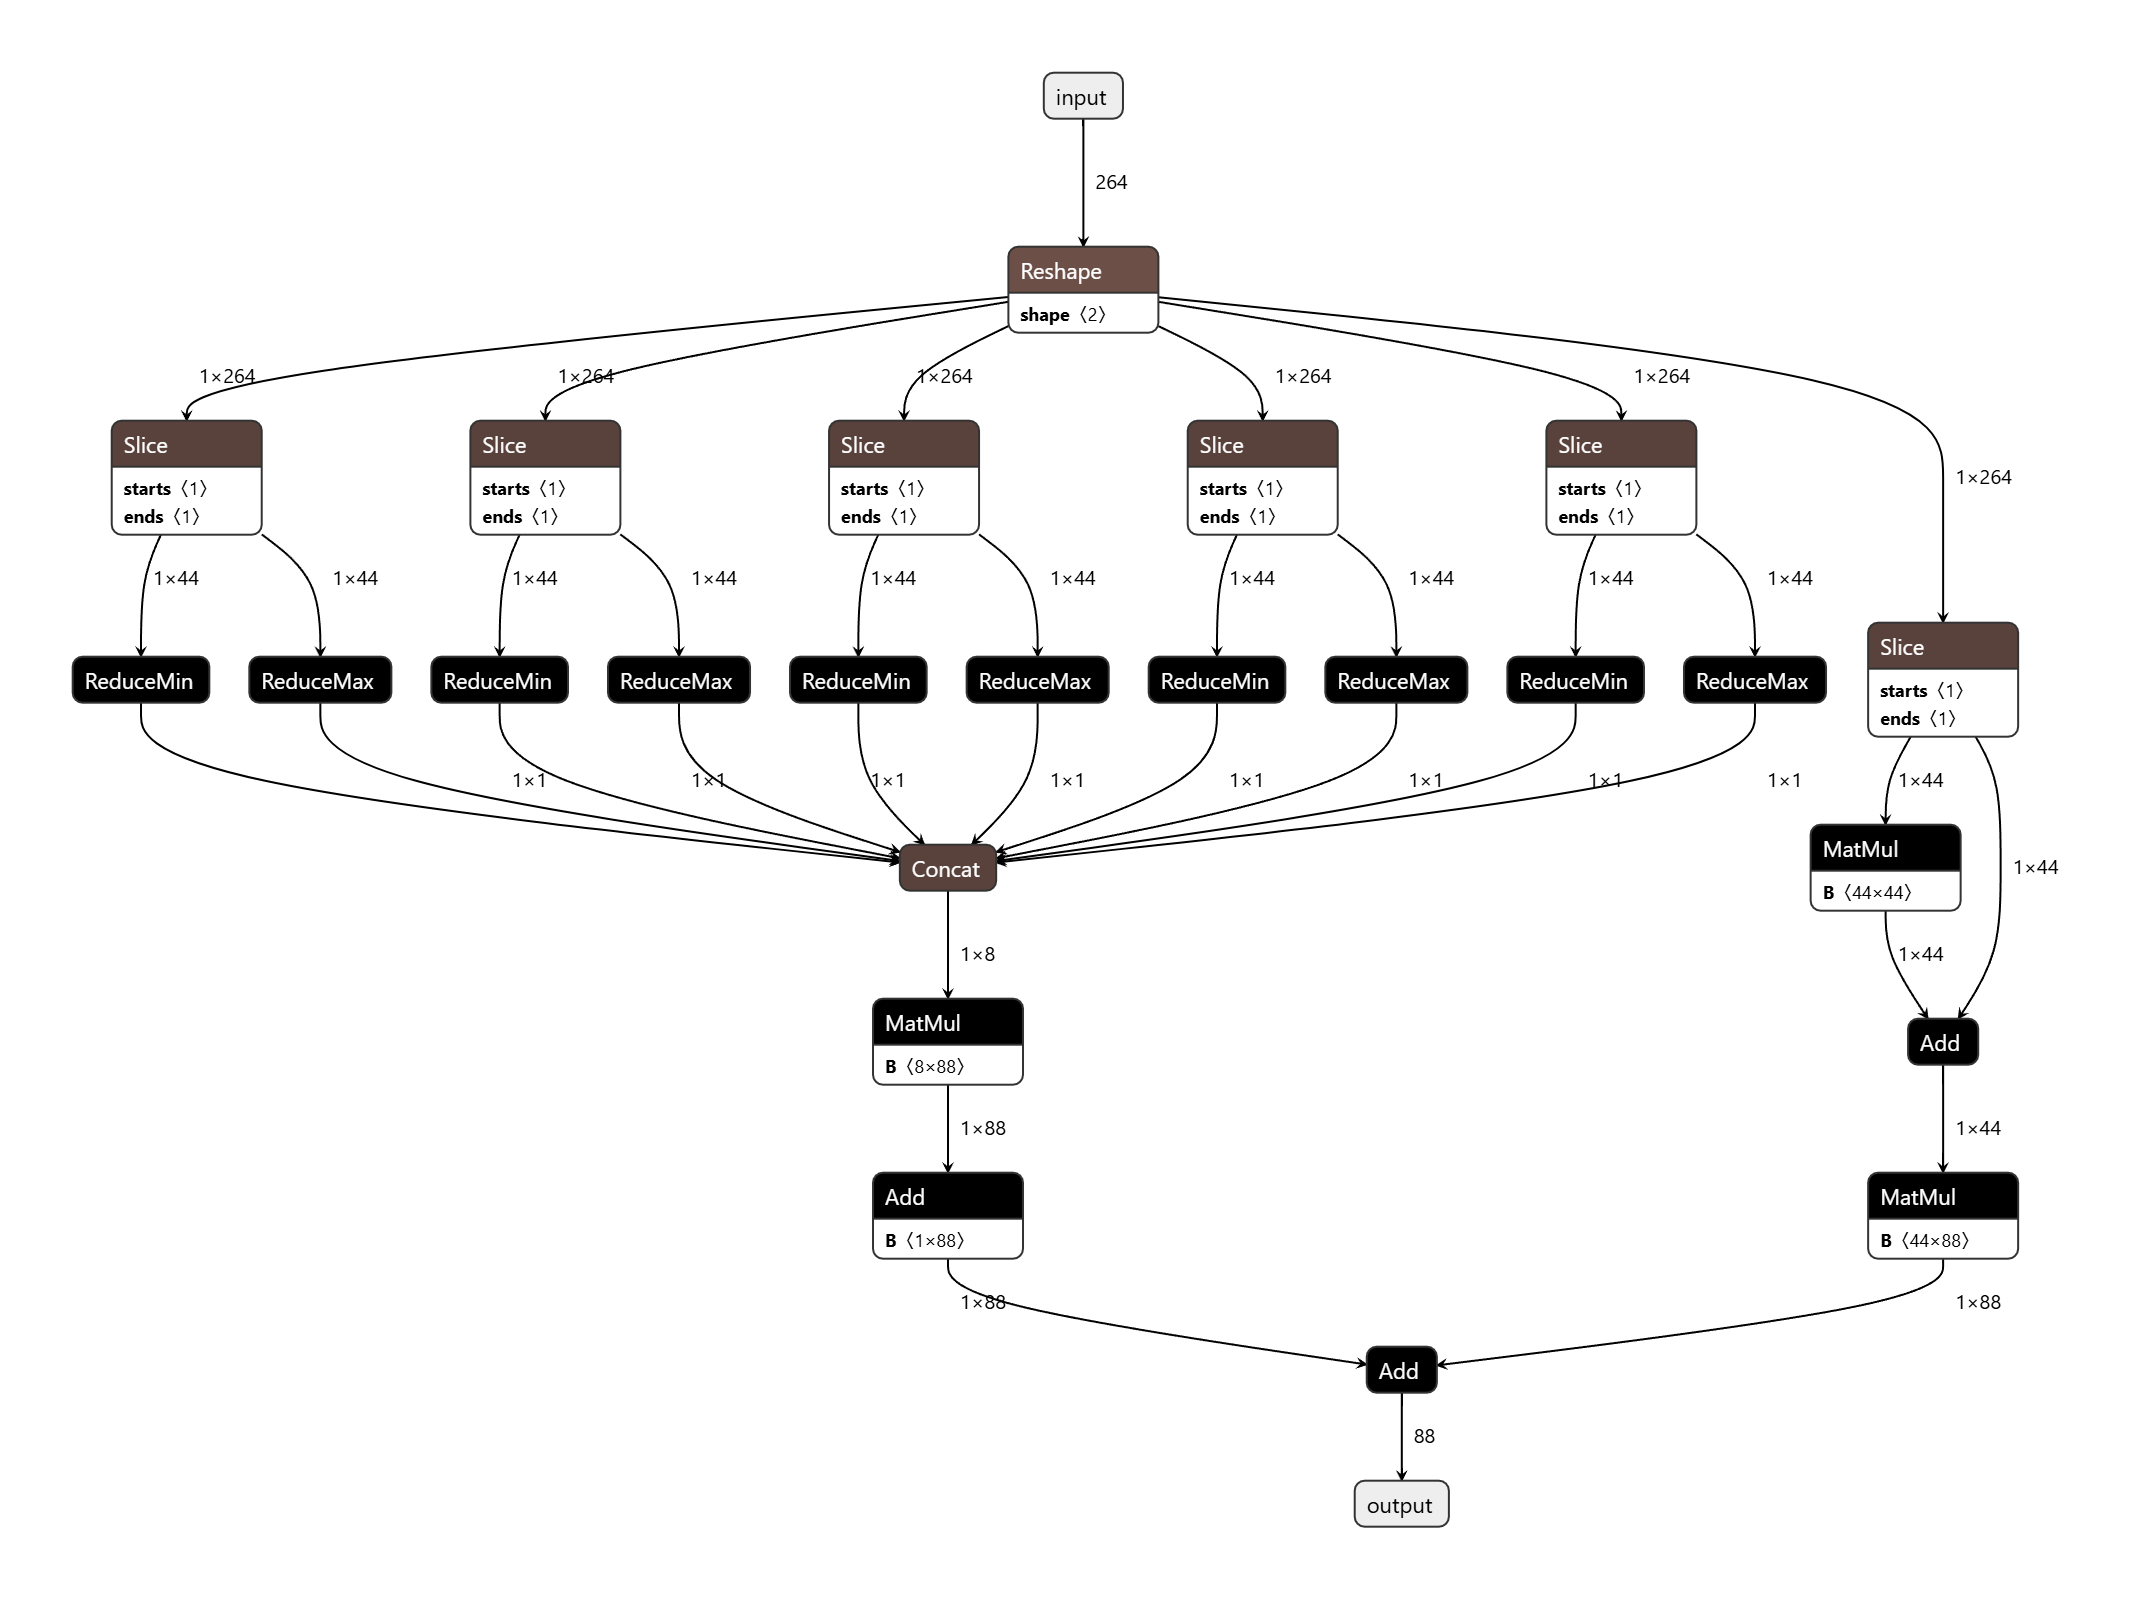
\includegraphics[width=1\textwidth]{image/chap02/custom_model.onnx.png}
    \caption{多分支因子模型样例}
    \label{fig:models}
\end{figure}


\section{模型推理框架}

在服务端高并发业务场景下,现有的多数推理框架侧重于处理大量请求的并行计算,通过分布式架构和异构计算来提高系统的吞吐量。
然而,低延时交易系统所面临的场景则截然不同,其优化的目标在于实现单样本高频率计算密集场景下的极低延时。
这就要求推理框架能够充分利用因子模型的结构特征与输入模式,通过针对性的优化策略,如内存映射、模型剪枝、算子融合等技术,有效提高模型整体的计算效率,降低推理延时。

当前多数模型推理框架仅针对服务端高并发场景进行了优化,对于高频交易的低延时要求缺乏针对性的解决方案。
然而即便优化的目的指标不同,现有推理框架的架构设计和技术应用对于低延时系统中的推理框架设计仍然具有参考意义。
例如,Tencent TFCC通过使用MLIR(多级中间表示)技术实现了自动算子融合,极大减小了由于算子编码调优而浪费的时间和人力,并显著降低了推理延时,
同时基于MLIR的Pass机制具有极强的可拓展性,Pass之间彼此解耦合,具有极高的优化上限。
llama.cpp则作为一个高度优化的C/C++实现,专注于本地LLM推理性能的优化,充分利用了现代CPU架构中的SIMD指令集,为多个LLM工具和应用提供了基础运行时支持,
其使用Protobuf作为模型的解析器,通过C++将模型进行进一步的包装和抽象,拓展了模型结构,同时为进一步优化提供开发空间。
TensorRT是NVIDIA推出的一个高性能深度学习推理优化器和运行时引擎,其包括静态计算图优化和动态推理优化两个解耦合的基本过程,
其静态计算图优化过程向上对模型适配,而动态推理优化过程向下对硬件适配,在取得优越性能的同时为推理框架设计提供了良好的启发。

除了现有模型推理框架的架构设计和技术应用外,因子模型的推理框架还应当面向系统和硬件做出针对性优化。
例如,在推理的执行过程中,缺页中断将导致严重的延时增长,因此使用大页的内存映射和内存锁定方法,能够在系统运行全过程内不发生缺页中断,有效提高访存性能。
利用系统调度指定CPU核心隔离操作,可以尽可能减少无关进程在指定核心的运行,从而有效提高CPU的占用时间。
在这些推理框架中,面向硬件的优化也是一个关键环节。
在日志系统的计时过程中,使用rdtscp指令计数器参与计时,能够以多核一致性clock的细粒度进行计时,完成高精度的性能测试。
通过针对特定硬件架构的算子实现,可以充分利用硬件的并行计算能力,提高计算效率。

总体来看,在模型推理框架的整体设计上,应当效仿先进的架构设计和技术应用,这将有效提高优化手段的效果上限。
同时在具体的内存管理和系统配置等方面,也要充分利用相关系统属性进行优化以提高访存和计算效率。
只有在综合多种优化手段的前提下,模型推理框架才能够在高频交易的低延时环境下有优越的性能表现。

\section{CPU计算体系}

尽管当前模型推理的硬件设备以GPU为主,但以业内普遍使用的英伟达A100计算卡为例,从CPU发起核函数到GPU执行核函数之间的延时就高达2.59微秒,而连续核函数之间的间隔延时约为5微秒(引用)。
而在更早的特斯拉架构中,发起矩阵乘操作核函数,其间隔延时高达20微秒,使其不具有应用价值。
\begin{figure}[h]
    \centering
    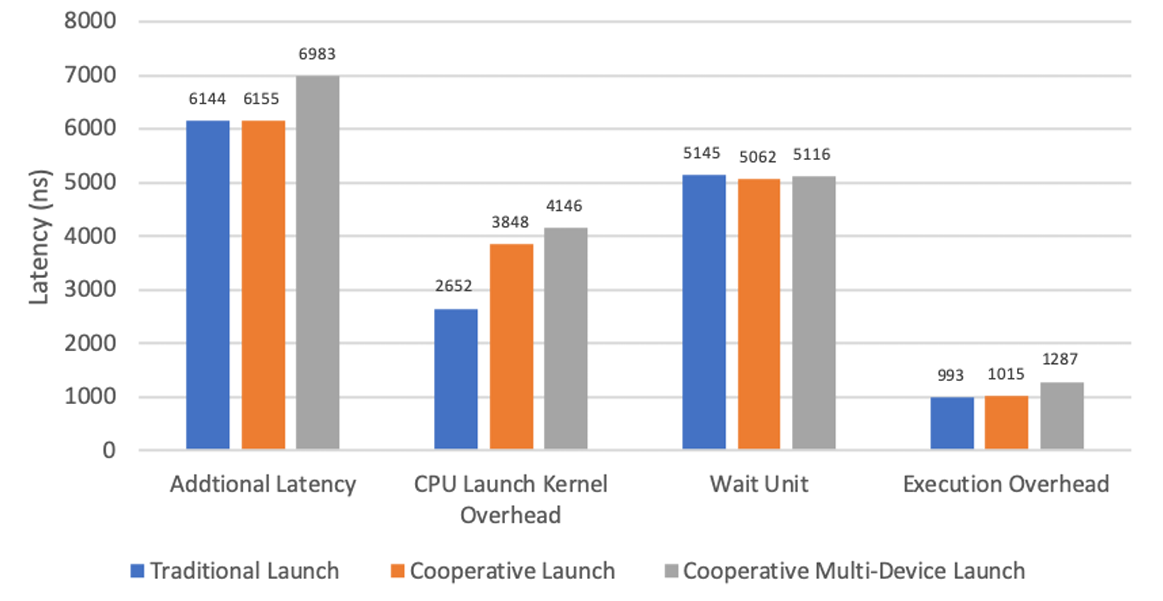
\includegraphics[width=1\textwidth]{image/chap02/Overhead.png}
    \caption{使用不同发起方法发起大型核函数的不同类型延时}
    \label{fig:kernel}
\end{figure}
如图\ref{fig:kernel}所示,在加入参数和数据传输后,延时已经使得因子模型在以期货市场为核心的高频交易中失去竞争力。
此外,尽管在多数工业计算场景如有限元计算中,计算过程通常被整体编码为一个核函数,
但对于时刻变化的业务模型,包括交易因子模型在内,为了维持项目的可读性和可维护性,不可避免地对计算节点进行抽象,进而将整个模型抽象为一个由算子组成的计算图。
在这种抽象计算图的推理过程中,算子核函数的连续发起导致仅累计启动延时就已超出预期。
因此,因子模型推理的目标硬件普遍使用服务器高性能多核CPU,尤其以AMD EPYC和Intel Xeon为业务主流硬件。

在高频交易场景下,CPU的性能对因子模型推理效率有着直接影响,优化方案必须根据CPU的架构进行针对性支持和优化。
当前主流的CPU架构中,EPYC和Xeon首先在核间访问延时方面存在较大差异。
EPYC架构采用了ccx和ccd设计,多个核心共享较大的L3缓存,适合处理多线程、大规模数据的计算任务,能够有效提高并行计算的效率。
但同时跨CCD通信往往需要占用CPU通信总线,因此可能导致较高的一致性延时。
而Xeon则采用了环路架构,核心之间通过环形总线进行通信,而与EPYC相比,环形总线具有更低的通信延时。
这种设计在单线程性能和跨核访存方面表现出色,能够快速处理高频率的单样本计算任务,更好地满足低延时交易系统的需求,
对应在高频交易从场景中,其广播延时和多播延时相较于EPYC有显著的改善。
两者在指令集支持方面也存在差异,这些差异决定了它们在不同计算场景下的适用性。
比如Xeon在支持AVX512指令集方面表现出良好的性能表现,而EPYC在一定时期内通过AVX2模拟AVX512实现兼容,此时在SIMD需求较高的应用中性能较差。
因此,CPU应当根据具体的业务场景配置指令集的使用以达到最优性能。
而充分利用不同CPU架构的特性,是能够有效改善推理过程延时的关键。

为了充分发挥CPU的计算能力,已有多种高性能计算库针对不同CPU架构做性能优化。
其中Intel MKL和AMD AOCL提供了面向Xeon和EPYC处理器的高效计算操作接口。
尤其是Intel MKL提供的GEMM JIT专注于矩阵计算的优化,通过即时编译技术生成针对特定矩阵尺寸和数据类型的高效计算代码,提高矩阵运算的性能。
Blaze HPC则是一个高效的数值计算库,通过将BLAS传入Blaze可以进一步根据CPU的指令集和各级缓存大小进行自动调优以达到最佳性能。
通过高度优化的算法和数据结构,Blaze HPC能够充分利用CPU的计算资源,加速数值计算过程。
Blaze HPC支持Tensor结构运算,这为因子模型推理框架提供了基本的高性能算子实现,使得CPU在高频交易场景下能够高效地完成复杂的计算任务。
